%=====================================================================
%  PREINFORME PRACTICA 2 - CONFIGURACIONES CON DIODOS
%  Electronica Analoga I - 2026-II - Universidad Nacional de Colombia
%
%  PARTE DEL INTEGRANTE 1 (version compacta: cabe en ~1-1.3 columnas
%  de IEEEtran a doble columna). Las subsecciones de los Integrantes
%  2 y 3 quedan comentadas en el ORDEN DE LA GUIA para que cada uno
%  pegue su texto sin romper numeracion de figuras/tablas/ecuaciones.
%  Recuerden: entre los tres NO deben superar 7 paginas sin contar
%  referencias, asi que redacten con el mismo nivel de compresion.
%
%  Compilar con pdfLaTeX. Se usan CINCO archivos de figura; subelos al
%  proyecto (en ./figuras/ o en la raiz, ambas rutas funcionan). Se
%  referencian SIN extension, asi que puedes reemplazar cualquiera por
%  una captura .png de LTspice con el mismo nombre:
%     CircuitoRectificadorFig1        (esquematico)
%     TransferenciaRectificadorFig1   (Vo vs Vi)
%     CircuitoMultiplicadorFig6       (esquematico, SINE(0 3 100))
%     SalidaMultiplicadorFig6         (Vo en el tiempo)
%     TransferenciaMultiplicadorFig6  (Vo vs Vi)
%=====================================================================
\documentclass[conference,10pt]{IEEEtran}

\usepackage[utf8]{inputenc}
\usepackage[T1]{fontenc}
\usepackage[spanish,es-nodecimaldot,es-noquoting]{babel}
\usepackage{amsmath,amssymb}
\usepackage{graphicx}
\usepackage{booktabs}
\usepackage{url}
\urlstyle{same}
\Urlmuskip=0mu plus 1mu\relax  % evita cajas subllenas en las URL

\graphicspath{{figuras/}{./}}   % busca en ./figuras/ y en la raiz

\begin{document}

\title{Configuraciones con diodos: rectificadores, limitadores,\\
sujetadores y multiplicadores de tensión}

\author{
\IEEEauthorblockN{Juan José Tobar Álvarez}
\IEEEauthorblockA{Departamento de Ingeniería Eléctrica y Electrónica\\
Universidad Nacional de Colombia\\
jutobara@unal.edu.co}
\and
\IEEEauthorblockN{Nombre Integrante 2}
\IEEEauthorblockA{Departamento de Ingeniería Eléctrica y Electrónica\\
Universidad Nacional de Colombia\\
correo2@unal.edu.co}
\and
\IEEEauthorblockN{Nombre Integrante 3}
\IEEEauthorblockA{Departamento de Ingeniería Eléctrica y Electrónica\\
Universidad Nacional de Colombia\\
correo3@unal.edu.co}
}

\maketitle

%=====================================================================
\section{Introducción y justificación}
% [INTEGRANTE 1 - version compacta]
%=====================================================================
El diodo $pn$ impone una dirección preferente a la corriente; de esa
propiedad se derivan las cuatro familias de circuitos de esta práctica:
rectificadores, limitadores, sujetadores y multiplicadores de
tensión~\cite{sedra}. El trabajo consiste en diseñar, simular y montar
ocho circuitos basados en la conmutación del diodo, contrastando el
modelo de caída constante $V_\gamma$ con los resultados de simulación.
Estas configuraciones no son solo académicas: la NASA rectificó y
convirtió 55~V CA de un sistema Brayton en 1100~V CC para alimentar el
propulsor iónico NSTAR con 91~\% de eficiencia~\cite{nasep}, y la celda
de la Fig.~\ref{fig:mult}(a) es la base de los multiplicadores
Cockcroft--Walton usados en fuentes de rayos X y de alta tensión sin
transformador~\cite{park}.

%=====================================================================
\section{Cálculos}
%=====================================================================

\subsection{Rectificadores: configuración, aplicaciones y limitaciones}
% [INTEGRANTE 1]
En media onda un diodo bloquea un semiciclo; en onda completa con
\textit{tap} central dos diodos conducen alternadamente sobre un
secundario dividido; en puente, cuatro diodos encaminan ambos
semiciclos con igual polaridad~\cite{sedra}. Se usan en la entrada de
fuentes CA/CC, cargadores y detectores de envolvente. Limitan su
desempeño la caída $V_\gamma$, la tensión inversa de pico (PIV), el
rizado, la zona muerta $|v_S|<V_\gamma$ y el tiempo de recuperación
inversa~\cite{vishay} (Tabla~\ref{tab:comp}).

\begin{table}[htbp]
\caption{Comparación de topologías rectificadoras ($V_m$: amplitud de
entrada; $V_\gamma$: caída directa; $f$: frecuencia de entrada).
$^1$Nodo compartido entre fuente y carga.}
\label{tab:comp}
\centering
\footnotesize
\setlength{\tabcolsep}{3.5pt}
\begin{tabular}{lccc}
\toprule
\textbf{Parámetro} & \textbf{Media onda} & \textbf{Tap central} & \textbf{Puente}\\
\midrule
$V_{o,\text{pico}}$      & $V_m-V_\gamma$   & $V_m-V_\gamma$      & $V_m-2V_\gamma$\\
$V_{DC}$ (ideal)         & $V_m/\pi$        & $2V_m/\pi$          & $2V_m/\pi$\\
$V_{\text{rms}}$ (ideal) & $V_m/2$          & $V_m/\sqrt{2}$      & $V_m/\sqrt{2}$\\
$f_o$ / PIV              & $f$ / $V_m$      & $2f$ / $2V_m{-}V_\gamma$ & $2f$ / $V_m{-}V_\gamma$\\
N.\ diodos / tierra$^1$  & 1 / Sí           & 2 / Sí              & 4 / No\\
\bottomrule
\end{tabular}
\end{table}

\subsection{Diseño del rectificador de onda completa (Fig. 1)}
% [INTEGRANTE 1]
Se requiere salida de amplitud $\approx5$~V y $f=1$~kHz. Se elige
\textit{tap} central (Tabla~\ref{tab:comp}: conserva tierra común) con
dos fuentes desfasadas $180^\circ$. Con caída constante,
$v_O=|v_S|-V_\gamma$, de donde

\begin{equation}
V_m=V_{o,\text{pico}}+V_\gamma=5+0.55=5.56\ \text{V}.
\label{eq:vm}
\end{equation}

Con $R_L=1$~k$\Omega$:
$I_{L,\text{pico}}=V_{o,\text{pico}}/R_L=5.01$~mA y
$\text{PIV}=2V_m-V_\gamma=10.57$~V, muy por debajo de los límites del
1N4004 ($I_{F(AV)}=1$~A, $V_{RRM}=400$~V)~\cite{vishay}. Los valores
teóricos ideal/con $V_\gamma$ se listan en la Tabla~\ref{tab:fig1}
(Fig.~\ref{fig:rect} muestra el circuito y su transferencia simulada).

\begin{figure}[htbp]
\centering
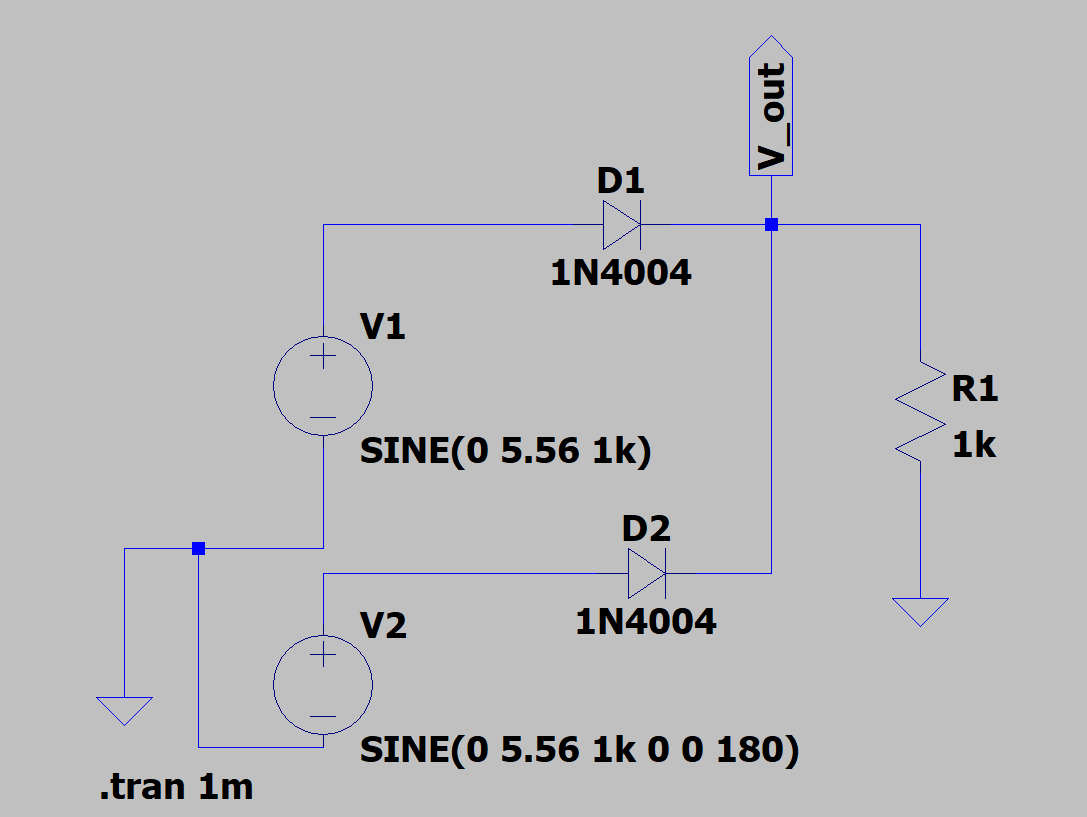
\includegraphics[width=0.5\columnwidth]{CircuitoRectificadorFig1}
\hfill
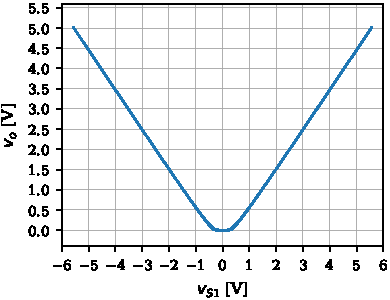
\includegraphics[width=0.44\columnwidth]{TransferenciaRectificadorFig1}
\caption{Rectificador de onda completa, \textit{tap} central
($V_m=5.56$~V, $f=1$~kHz, $R_L=1$~k$\Omega$): (a) circuito y (b)
transferencia simulada.}
\label{fig:rect}
\end{figure}

\subsection{Medición y condiciones de la señal de entrada}
% [INTEGRANTE 1 - las 3 preguntas de la Fig. 1, en formato compacto]
\textbf{Puente:} la carga queda flotante; medir simultáneamente entrada
y salida con tierras comunes cortocircuita diodos. Se requiere medida
diferencial o registros por separado.
\textbf{Entrada:} debe ser alterna, bipolar, con $V_m\gg V_\gamma$ y
frecuencia baja frente al inverso del $t_{rr}$ del diodo; en
\textit{tap} central ambas fuentes deben tener igual amplitud y desfase
exacto de $180^\circ$.
\textbf{Tierras:} en \textit{tap} central el punto medio es común a
fuente y carga (una sola referencia sirve para las dos puntas); en
puente no existe ese nodo, por lo que la medición simultánea exige
diferencial o aislamiento --- de ahí la preferencia por \textit{tap}
central en el montaje.

% ---------------------------------------------------------------
% [INTEGRANTE 2] \subsection{Limitadores: configuración, aplicaciones y limitaciones}
% [INTEGRANTE 2] \subsection{Diseño del rectificador de onda completa con filtro capacitivo (Fig. 2)}
% [INTEGRANTE 2] \subsection{Diseño del sujetador a +3 V (Fig. 3)}
% [INTEGRANTE 3] \subsection{Sujetadores y multiplicadores: configuración, aplicaciones y limitaciones}
% [INTEGRANTE 3] \subsection{Diseño del sujetador a -4 V (Fig. 4)}
% [INTEGRANTE 3] \subsection{Diseño del sujetador con recorte en +-4 V (Fig. 5)}
% ---------------------------------------------------------------

%=====================================================================
\section{Simulación}
%=====================================================================

\subsection{Multiplicador de tensión (Fig. 6)}
% [INTEGRANTE 1]
Simulado con $v(t)=3\sin(\omega t)$~V, 100~Hz, 100~ms
(Fig.~\ref{fig:mult}(a)). $C_1$--$D_1$ (cátodo a tierra) sujeta la
entrada entre $0$ y $-2V_m$; $D_2$--$C_2$ detecta ese pico, así que en
régimen permanente

\begin{equation}
V_O\approx-2\left(V_m-V_\gamma\right)=-5.1\ \text{V},
\label{eq:doblador}
\end{equation}

un \textbf{doblador de tensión de media onda, salida negativa}
(Cockcroft--Walton elemental). La Fig.~\ref{fig:mult}(b) muestra la
salida creciendo en escalones (uno por ciclo) hasta $-5.12$~V
(0.5~\% sobre \eqref{eq:doblador}; 14.6~\% bajo el ideal $-2V_m$). El
rizado, $r=V_{r(pp)}/(2\sqrt3|V_{DC}|)\times100$, se resume en la
Tabla~\ref{tab:mult}.

\begin{figure}[htbp]
\centering
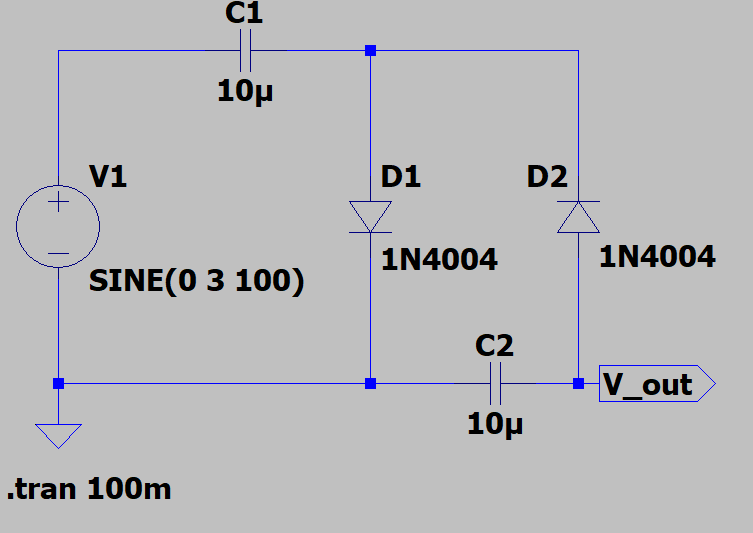
\includegraphics[width=0.55\columnwidth]{CircuitoMultiplicadorFig6}\\[2pt]
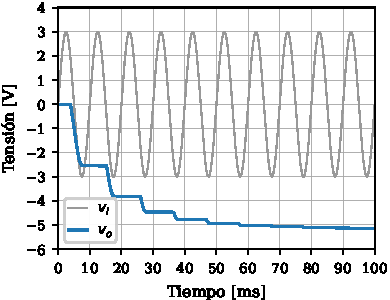
\includegraphics[width=0.48\columnwidth]{SalidaMultiplicadorFig6}
\hfill
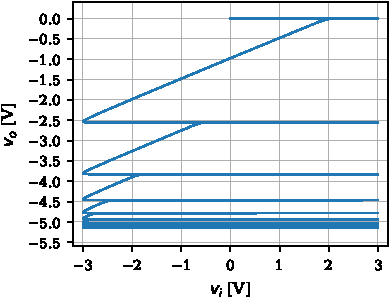
\includegraphics[width=0.48\columnwidth]{TransferenciaMultiplicadorFig6}
\caption{Multiplicador ($C_1{=}C_2{=}10\,\mu$F, 1N4004,
$v(t){=}3\sin(\omega t)$~V, 100~Hz): (a) circuito, (b) salida en el
tiempo, (c) transferencia $v_o$--$v_i$.}
\label{fig:mult}
\end{figure}

\begin{table}[htbp]
\caption{Multiplicador, $V_m=3$~V (teórico: $-5.10$~V; ideal: $-6.00$~V).}
\label{tab:mult}
\centering
\footnotesize
\setlength{\tabcolsep}{4pt}
\begin{tabular}{ccccc}
\toprule
$f$ [Hz] & $V_{o,DC}$ [V] & $V_{r(pp)}$ [mV] & $r$ [\%] & $t_{95\%}$ [ms]\\
\midrule
100  & $-5.12$ & 45.7 & 0.257 & 47.3\\
1000 & $-5.21$ & 24.7 & 0.137 & 11.8\\
\bottomrule
\end{tabular}
\end{table}

\subsection{Identificación por la función de transferencia}
% [INTEGRANTE 1]
En la Fig.~\ref{fig:mult}(c) la curva $v_o$--$v_i$ no es univaluada:
segmentos casi horizontales colapsan en $v_o\approx-5.12$~V, con
$|v_o|>V_m$. Ese es el criterio: un \textit{rectificador} da una curva
univaluada por el origen (recta a $45^\circ$ o ``V'', Fig.~\ref{fig:rect}(b));
un \textit{limitador}, pendiente unitaria con mesetas de recorte; un
\textit{sujetador}, recta de pendiente unitaria desplazada
verticalmente; solo el \textit{multiplicador} pierde la dependencia con
el valor instantáneo de $v_i$ (la fija la carga de los condensadores) y
su transferencia degenera en una recta horizontal con $|v_o|>V_m$.

\subsection{Efecto de frecuencia y amplitud}
% [INTEGRANTE 1]
A 1~kHz (Tabla~\ref{tab:mult}) el rizado baja de 45.7 a 24.7~mV y el
establecimiento de 47.3 a 11.8~ms, porque el intervalo de descarga entre
picos se reduce diez veces. Por \eqref{eq:doblador}, $|V_O|$ escala
linealmente con $V_m$; si $V_m\to V_\gamma$ los diodos dejan de
conducir y la multiplicación desaparece (de ahí la ganancia efectiva
1.71 en vez de 2).

\subsection{Verificación del rectificador de onda completa (Fig. 1)}
% [INTEGRANTE 1 - coordinar con Integrante 2, numeral 4.2.2]
La Tabla~\ref{tab:fig1} contrasta diseño y simulación: 5.01~V de pico,
período 0.5~ms (el doble de la entrada, como corresponde a onda
completa), y $V_{DC}$/$V_{\text{rms}}$ dentro del 1.1~\% del modelo con
$V_\gamma$. La Fig.~\ref{fig:rect}(b) exhibe además la zona muerta
$\pm0.35$~V en torno al origen.

\begin{table}[htbp]
\caption{Rectificador de onda completa ($V_m=5.56$~V, $f=1$~kHz,
$R_L=1$~k$\Omega$): cálculo contra simulación.}
\label{tab:fig1}
\centering
\footnotesize
\setlength{\tabcolsep}{3.5pt}
\begin{tabular}{lcccc}
\toprule
\textbf{Parámetro} & \textbf{Ideal} & \textbf{Teórico} & \textbf{LTspice} & \textbf{Err.}\\
 & $V_\gamma{=}0$ & $V_\gamma{=}0.55$~V & & [\%]\\
\midrule
$V_{o,\text{pico}}$ [V] & 5.56 & 5.01 & 5.01 & 0.04\\
$V_{DC}$ [V]            & 3.54 & 3.01 & 3.04 & 1.06\\
$V_{\text{rms}}$ [V]    & 3.93 & 3.44 & 3.46 & 0.35\\
$f_{o}$ [kHz] / PIV [V] & 2.00/11.12 & 2.00/10.57 & 2.00/--- & 0/---\\
\bottomrule
\end{tabular}
\end{table}

% ---------------------------------------------------------------
% [INTEGRANTE 2] \subsection{Simulación de las Figuras 1 y 2 y comparación con los cálculos}
% [INTEGRANTE 3] \subsection{Simulación de las Figuras 3, 4 y 5 y comparación con los cálculos}
% [INTEGRANTE 3] \subsection{Diseño a partir de las funciones de transferencia (Figuras 7a y 7b)}
% [INTEGRANTE 3] \subsection{¿Pueden conducir simultáneamente los dos diodos del limitador?}
% ---------------------------------------------------------------

%=====================================================================
\section{Montaje}
%=====================================================================
% Se completa el dia de la practica (numeral 5): montaje de los ocho
% circuitos en protoboard e imagenes de entrada/salida del osciloscopio.
Esta sección se desarrollará durante la sesión de laboratorio.

%=====================================================================
\section{Análisis de resultados}
%=====================================================================
% [INTEGRANTE 1 - version compacta]
El error entre el cálculo ideal y la simulación (Tabla~\ref{tab:fig1})
proviene del modelo del diodo: sin $V_\gamma$ se sobreestima $V_{DC}$ en
16~\%, y con $V_\gamma$ constante el error baja a 1~\%; el remanente se
debe a que el modelo SPICE es exponencial (la caída pasa de 0.50~V a
1.5~mA a 0.55~V a 5~mA). El mismo efecto explica el multiplicador: la
diferencia entre $-6$~V ideales y $-5.12$~V simulados son las dos caídas
directas, pero la caída equivalente es menor (0.44~V) porque en régimen
permanente solo circula corriente de fuga, la cual también sostiene el
rizado residual de la Tabla~\ref{tab:mult} pese a no haber carga
resistiva.
% [PENDIENTE tras el laboratorio: comparar mediciones de osciloscopio y
%  multímetros (DC, RMS) con las Tablas III y IV.]

%=====================================================================
\section{Conclusiones}
%=====================================================================
% [INTEGRANTE 1 - se integran con las de los demas]
\begin{itemize}
\item Compensar $V_\gamma$ en la amplitud de fuente ($V_m=5.56$~V) dio
una salida de 5.01~V, 0.2~\% por debajo de los 5~V pedidos: el modelo de
caída constante sirve para diseñar, no solo para analizar.
\item El \textit{tap} central se prefirió por conservar tierra común
fuente--carga, evitando medida diferencial o aislamiento en el
osciloscopio de doble traza.
\item La Fig.~6 es un doblador de salida negativa ($-5.12$~V simulados
frente a $-5.10$~V teóricos); su transferencia no univaluada con
$|v_o|>V_m$ la distingue de rectificador, limitador y sujetador.
\item Subir de 100~Hz a 1~kHz redujo el rizado de 0.257 a 0.137~\% y el
establecimiento de 47.3 a 11.8~ms: la frecuencia controla la calidad de
la continua obtenida en circuitos con condensador.
\end{itemize}

%=====================================================================
\begin{thebibliography}{9}
%=====================================================================
\bibitem{sedra}
A. S. Sedra, K. C. Smith, T. C. Carusone y V. Gaudet, \emph{Microelectronic
Circuits}, 8.ª ed. Nueva York, NY, EE.UU.: Oxford University Press, 2020.

\bibitem{nasep}
National Academies of Sciences, Engineering, and Medicine, \emph{Space
Nuclear Propulsion for Human Mars Exploration}. Washington, DC, EE.UU.:
The National Academies Press, 2021. [En línea]. Disponible:
\url{https://www.nationalacademies.org/read/25977/chapter/5}

\bibitem{park}
S. Park, J. Yang y J. Rivas-Davila, ``A hybrid Cockcroft--Walton/Dickson
multiplier for high voltage generation,'' \emph{IEEE Trans. Power
Electron.}, 2019. [En línea]. Disponible:
\url{https://par.nsf.gov/servlets/purl/10106507}

\bibitem{vishay}
Vishay General Semiconductor, ``1N4001 thru 1N4007: General purpose
plastic rectifier,'' hoja de datos, 2023. [En línea]. Disponible:
\url{https://assets.rs-online.com/v1698967669/Datasheets/13e6e46c15cf22864bd07ab7e9c4439c.pdf}

\end{thebibliography}

\end{document}
